\subsection{Sensors}
\subsubsection{Introduction}
The microAmpere platform is equipped with a wide range of sensors supporting navigation, perception, and control tasks. For this work, the focus lies on the integration of a Side Scan Sonar and the development of an \todo{TAP: what does SSS stand for?}<SSS SLAM. Two of the existing sensors play a key role in enabling this, the Inertial Measurement Unit (IMU) and the Global Navigation Satellite System (GNSS). These sensors together provide accurate state estimation and position tracking, forming the foundation required for precise sonar data alignment, georeferencing, and mapping.



\subsubsection{Inertial Measurement Unit (IMU) for Navigation and Pose Estimation}
\noindent
The \textit{``Sensonor STIM300''} is the primary Inertial Measurement Unit (IMU) onboard microAmpere. It is a tactical grade sensor providing precise angular rate and linear acceleration measurements for dead reckoning, attitude estimation, and control stabilization. Its compact and rugged design makes it well suited for marine robotics, where vibration, temperature variation, and magnetic disturbances are common. The unit integrates three high precision gyroscopes and three accelerometers, enabling full 3-axis motion sensing with excellent mechanical and thermal stability.
\\ \\
The STIM300 offers a $\pm400~^{\circ}/s$ gyroscope range and $\pm10~g$ accelerometer range with 24-bit resolution, ensuring low noise and stable long term performance. It communicates via an RS-422 interface, operates from a 5~V supply, and supports sampling rates up to 2~kHz with deterministic timing. Its low bias instability and minimal drift allow reliable short term dead reckoning when GNSS signals are unavailable, making it a key component for autonomous control and future side scan sonar-based SLAM integration.
\\ \\
An overview of the IMU is shown in Figure \ref{fig:microAmpere-imu}, and its key specifications are summarized in Table \ref{tab:IMU-specs}.
\begin{figure}[H]
    \centering
    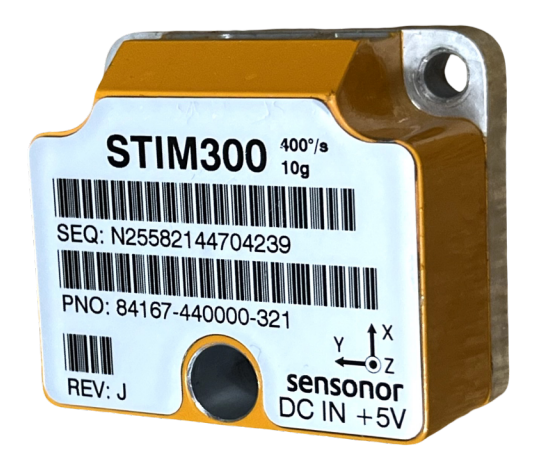
\includegraphics[width=0.45\linewidth]{Pictures/Hardware/Sensors/IMU.png}
    \caption{Sensonor STIM300 high-performance IMU used for internal navigation and pose estimation. Picture taken from Henrik Reimers master thesis on microAmpere ASV.\textsuperscript{\cite{microAmpere_hardware_master_thesis1}}}
    \label{fig:microAmpere-imu}
\end{figure}

\begin{table}[H]
    \centering
    \caption{Sensonor STIM300 IMU specifications summary.\textsuperscript{\cite{imu_data_sheet}}}
    \label{tab:IMU-specs}
    \begin{tabular}{lc}
        \hline
        \textbf{Parameter} & \textbf{Value} \\
        \hline
        Gyroscope range & $\pm400~^{\circ}/s$ \\
        Accelerometer range & $\pm10~g$ \\
        Resolution & 24-bit \\
        Max data rate & 2~kHz \\
        Interface & RS-422 \\
        Input voltage & 5~V \\
        Weight & 55~g \\
        \hline
    \end{tabular}
\end{table}



\newpage



\subsubsection{GNSS for Positioning and Heading Estimation}
For accurate positioning and heading estimation, microAmpere employs two \textit{``u-blox ZED-F9P''} GNSS modules integrated on a Dual GNSS card from SentiSystems. These modules support Real-Time Kinematic (RTK) corrections for centimeter level positioning accuracy and operate in a moving base configuration to estimate heading from the relative position of two GNSS antennas.
\\ \\
The external \textit{``SignalPlus''} GNSS antennas provide reliable satellite reception and minimize multipath effects common in harbor environments. With a baseline distance of approximately 0.7m between antennas, the system achieves heading accuracy of around 0.5\textdegree{}, while maintaining position accuracy down to 1.5m, or 0.01m with RTK corrections. This configuration ensures precise navigation and robust performance even under challenging marine conditions.
\\ \\
Together with the onboard IMU, the dual GNSS system forms the foundation for the vessels navigation, control, and future SSS SLAM integration. The Dual GNSS card and antennas are shown in Figure \ref{fig:microAmpere-gnss}, and the system specifications are summarized in Table \ref{tab:GNSS-specs}.
\begin{figure}[H]
    \centering
    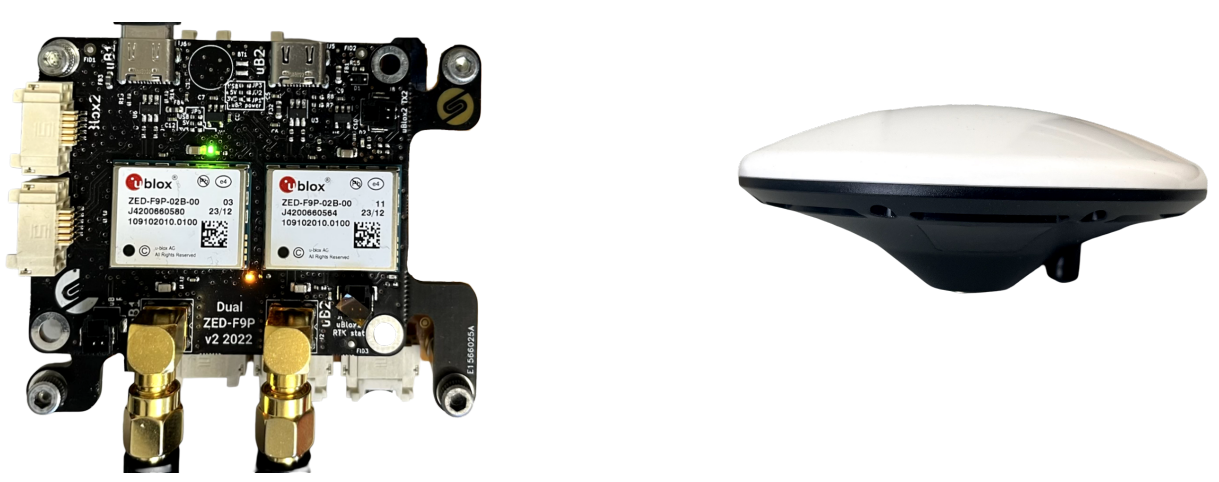
\includegraphics[width=0.9\linewidth]{Pictures/Hardware/Sensors/GNSS_Card_and_GNSS_Antenna.png}
    \caption{(Left) SentiSystems Dual GNSS card with two u-blox ZED-F9P modules. (Right) SignalPlus GNSS antennas used for position and heading estimation. Picture taken from Henrik Reimers master thesis on microAmpere ASV.\textsuperscript{\cite{microAmpere_hardware_master_thesis1}}}
    \label{fig:microAmpere-gnss}
\end{figure}

\begin{table}[H]
    \centering
    \caption{GNSS module specifications summary.\textsuperscript{\cite{gnss_data_sheet}}}
    \label{tab:GNSS-specs}
    \begin{tabular}{lc}
        \hline
        \textbf{Parameter} & \textbf{ZED-F9P} \\
        \hline
        Position accuracy (CEP) & 1.5~m (0.01~m with RTK) \\
        Heading accuracy & 0.4\textdegree~(baseline 1.8~m) \\
        RTK capability & Base + Moving Base \\
        Satellite bands & L1, L2, L5 \\
        Max navigation rate & 25~Hz (5~Hz moving base) \\
        \hline
    \end{tabular}
\end{table}



\newpage



\subsubsection{Side Scan Sonar for Environmental Perception and SLAM}
The \textit{``DeepVision OSM Ethernet Sonar System''} is the side scan sonar used onboard the microAmpere platform for seabed imaging, mapping, and SLAM development. Developed by DeepVision AB, this system operates with dual 680~kHz transducers utilizing chirp modulation to produce high resolution acoustic imagery. It supports a maximum operating depth of 100~m and can achieve image resolutions down to 1~cm depending on configuration settings.
\\ \\
The OSM sonar was previously evaluated by Hogstad, Bjørnar Reitan in his masters thesis at NTNU, where it was integrated on a BlueROV2 platform with an Error State Kalman Filter (ESKF) for autonomous navigation and acoustic mapping \cite{side_scan_sonar_master_thesis_old}. In that setup, the transducers were mounted symmetrically and angled downward at $\theta = 45^{\circ}$, providing a vertical beam width of $\alpha = 60^{\circ}$ and a horizontal beam width of $\phi = 0.7^{\circ}$. This configuration allowed both wide area coverage and high spatial resolution across the seafloor.
\\ \\
The sonar connects via Ethernet to the onboard computer and is automatically recognized by the \textit{``DeepView LT''} software for real-time imaging, control, and data logging. Its high operating frequency and narrow horizontal beam enable precise seafloor mapping, while the wide vertical beam ensures efficient coverage for environmental perception. This makes it highly suitable for integration into the microAmpere ASVs perception stack, supporting the development of SSS SLAM and environment aware autonomy.
\\ \\
An overview of the sonar system is shown in Figure \ref{fig:microAmpere-side-scan-sonar}, and its main specifications are summarized in Table \ref{tab:side-scan-sonar-specs}.
\begin{figure}[H]
    \centering
    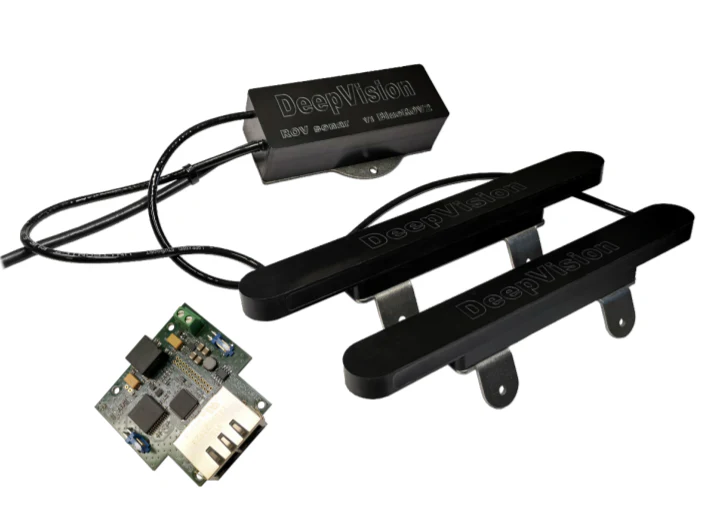
\includegraphics[width=0.5\linewidth]{Pictures/Hardware/Sensors/Side_Scan_Sonar.png}
    \caption{DeepVision OSM Ethernet Side-Scan Sonar system with dual 680~kHz transducers used for seabed imaging and SLAM development. Picture adapted from Hogstads master thesis on BlueROV2 sonar integration.\textsuperscript{\cite{side_scan_sonar_master_thesis_old}}}
    \label{fig:microAmpere-side-scan-sonar}
\end{figure}

\begin{table}[H]
    \centering
    \caption{DeepVision OSM Ethernet Sonar System specifications summary.\textsuperscript{\cite{side_scan_sonar_master_thesis_old}}}
    \label{tab:side-scan-sonar-specs}
    \begin{tabular}{lc}
        \hline
        \textbf{Parameter} & \textbf{Value} \\
        \hline
        Operating frequency & 680~kHz (Chirp signal) \\
        Resolution & Down to 1~cm \\
        Maximum operating depth & 100~m \\
        Vertical beam width ($\alpha$) & 60\textdegree \\
        Horizontal beam width ($\phi$) & 0.7\textdegree \\
        Mounting angle ($\theta$) & 45\textdegree \\
        Swath range & Up to 50~m per side (100~m total) \\
        Interface & Ethernet \\
        Software & DeepView LT \\
        Manufacturer & DeepVision AB \\
        \hline
    \end{tabular}
\end{table}
